\subsection{W-WC-DCGAN}
\label{sec:exp-w-wc-dcgan}
We implement weight clipping (WC) on top of the W-DCGAN from the previous section. As stated before, the authors of WGAN state that this method is a far from ideal way to ensure a norm on the gradients. However, we still expect it to outperform the W-DCGAN. We present the evolution of the Inception score and losses in Figures \ref{fig:exp-w-wc-dcgan-is} and \ref{fig:exp-w-wc-dcgan-losses}, respectively. %
\begin{figure}[H]
    \centering
    \begin{subfigure}[t]{0.49\textwidth}
        \centering
		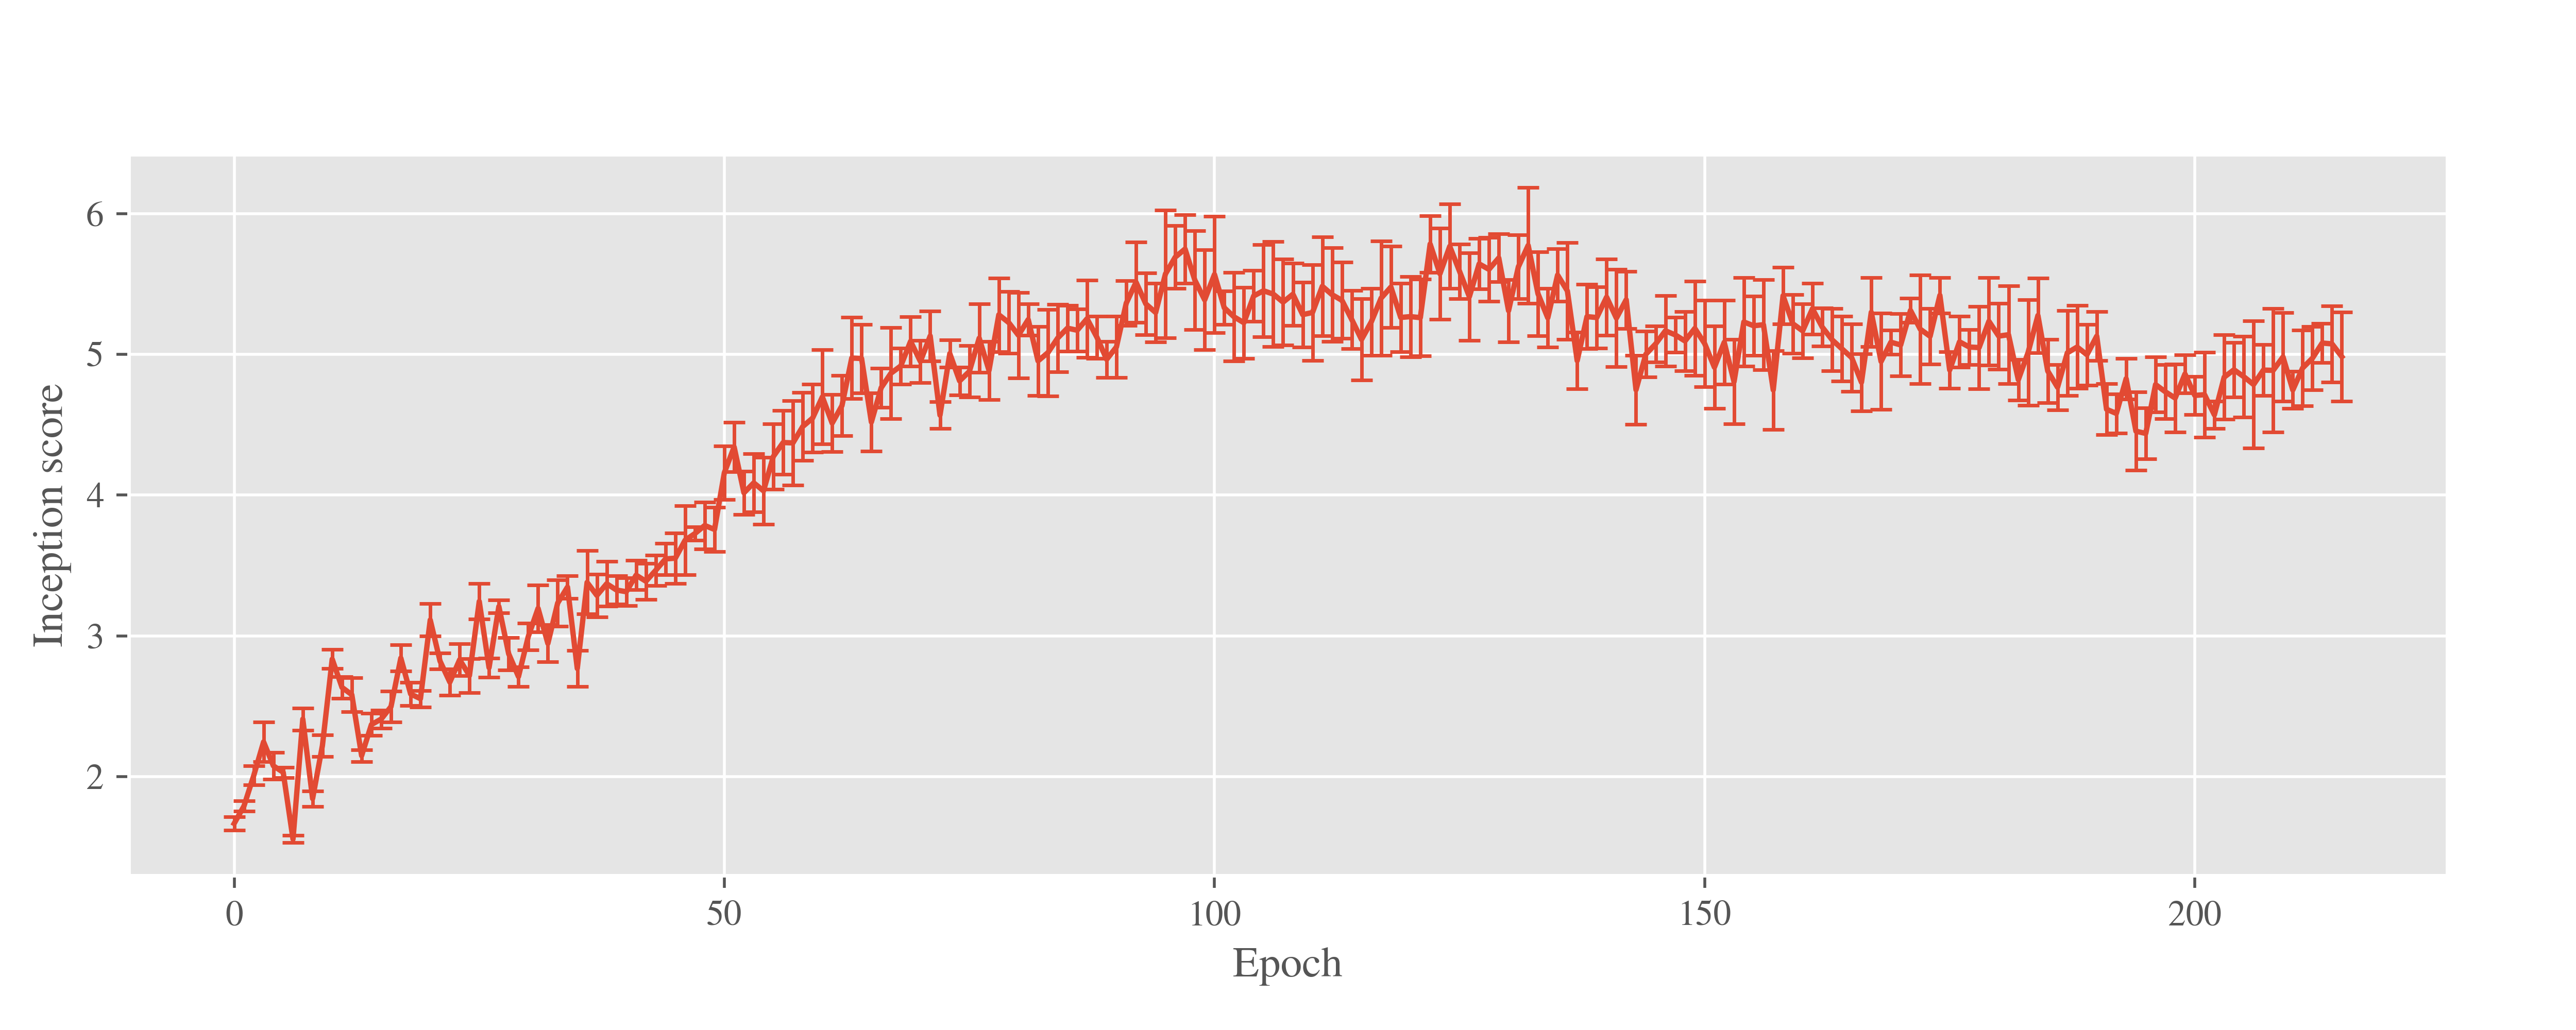
\includegraphics[width=\textwidth]{../code/results/figures/w-wc-dcgan_cifar10_is.png}
		\caption{Inception score}
		\label{fig:exp-w-wc-dcgan-is}
    \end{subfigure}
    \begin{subfigure}[t]{0.49\textwidth}
        \centering
        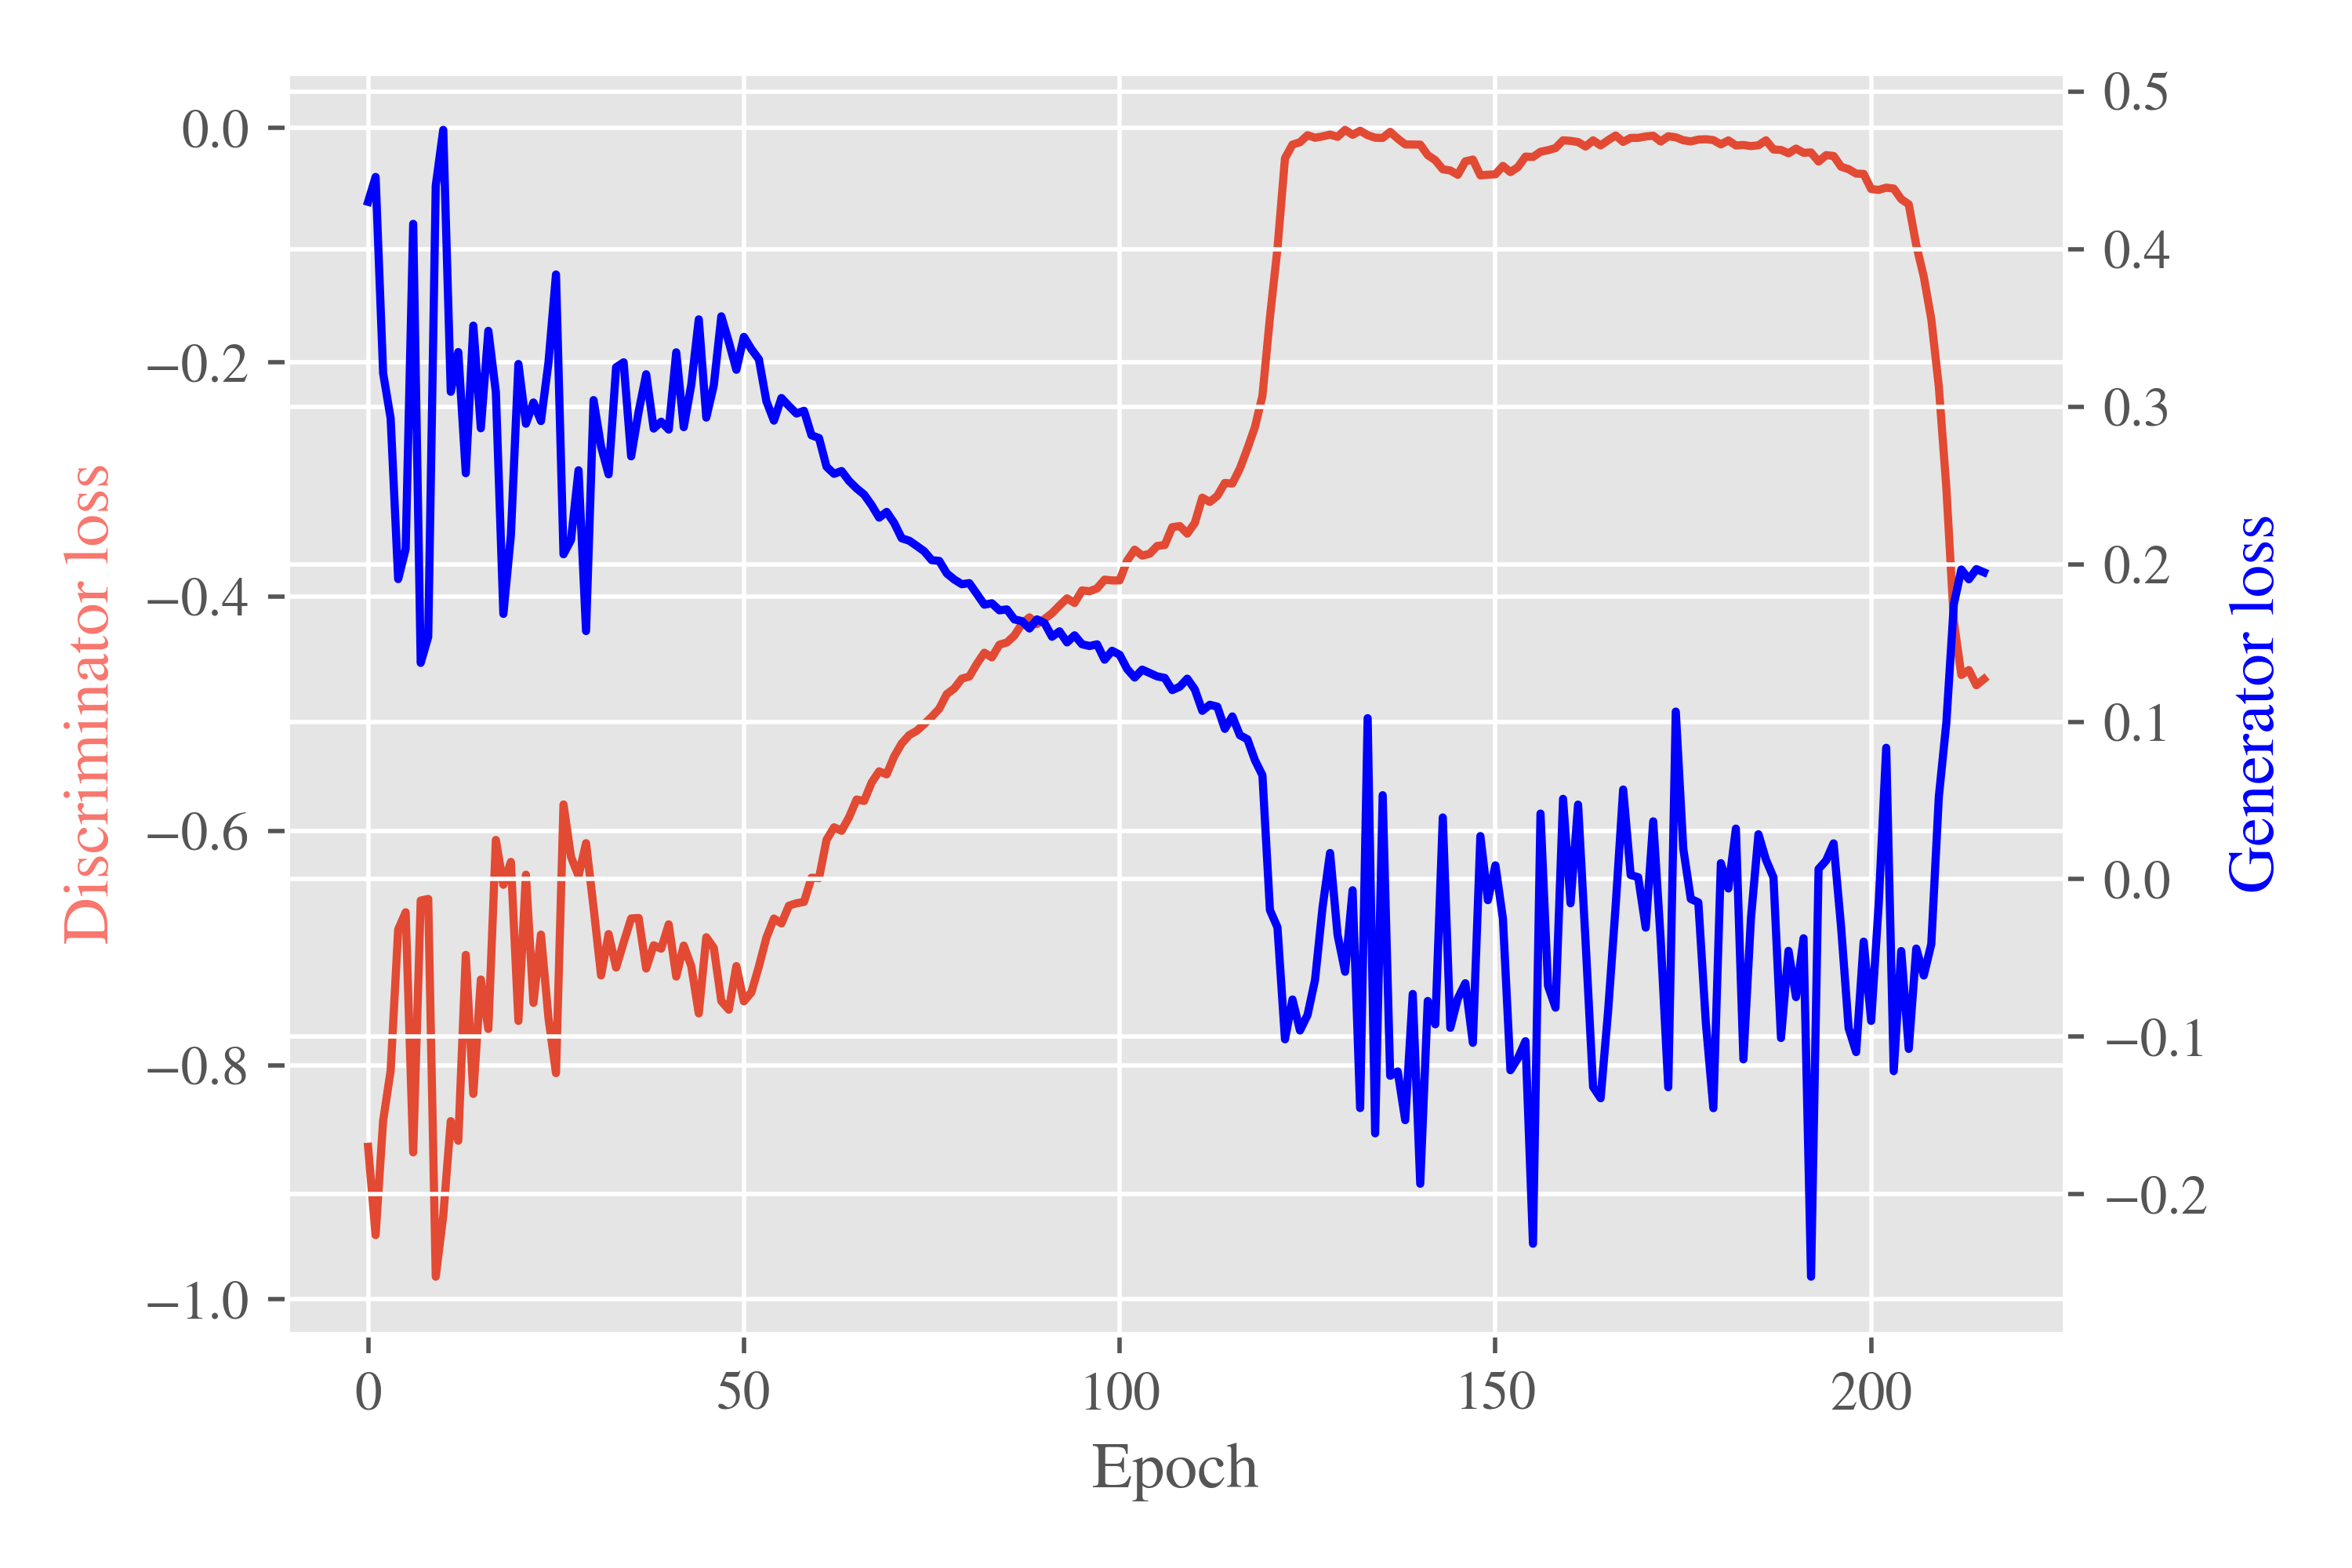
\includegraphics[width=\textwidth]{../code/results/figures/w-wc-dcgan_cifar10_losses.png}
		\caption{Losses}
		\label{fig:exp-w-wc-dcgan-losses}
    \end{subfigure}
    \caption{W-WC-DCGAN - training on CIFAR10 over 200 epochs.}
\end{figure}%
We observe a turbulent climb for the Inception score and an even more chaotic evolution of the losses. Looking at the losses, it seems like the training has two different ``regimes''. We propose an interpretation, even though we cannot be sure of its accuracy. In all experiments, we initialize weights by sampling from a Normal distribution with mean 0 and standard deviation 0.02. Here, we use the recommended clipping value of 0.01 \cite{arjovsky2017wasserstein}. This means that for the first iterations, most weights are systematically clipped, and possibly by a lot. It is easy to think how this would lead to unpredictable or unstable behaviour, seemingly experienced in epochs 0 to 50. Then, we think that weights enter a range that suits the requirements of WGAN, leading to a more stable training phase until epoch 120. After this epoch, the generator seems to enter a new chaotic regime, possibly because the discriminator reached a well performing region where it becomes hard to fool. This problem might be solved with thorough hyper-parameter tuning.